\chapter{Liveness Analysis of Intermediate Values}

The maintenance of intermediate values during expression evaluation in
the Icon programming language is more complicated than it is for
conventional languages such as C and Pascal. O'Bagy explains this in
her dissertation [.tr88-31.]:

\begin{quote}
``Generators prolong the lifetime of temporary values. For example, in 

\iconline{\>\>i = find(s1,s2)}

\noindent
the operands of the comparison operation cannot be discarded when
\texttt{find} produces its result. If \texttt{find} is resumed, the
comparison is performed again with subsequent results from
\texttt{find(s1,s2}), and the left operand must still be available.''
\end{quote}

\noindent In some implementation models, it is equally important that
the operands of \texttt{find} still be available if that function is
resumed (this depends on whether the operand locations are used during
resumption or whether all needed values are saved in the local state
of the function).

As noted in Chapter 14, a stack-based model handles the lifetime
problem dynamically. However, a temporary-variable model like the one
used in this compiler requires knowledge at compile-time of the
lifetime of intermediate values. In a straightforward implementation
of conventional languages, liveness analysis of intermediate values is
trivial: an intermediate value is computed in one place in the
generated code, is used in one place, and is live in the contiguous
region between the computation and the use. In such languages,
determining the lifetime of intermediate values only becomes
complicated when certain optimizations are performed, such as code
motion and common subexpression elimination across basic blocks
[.dragonbk,progflw.]. This is not true in Icon. In the presence of
goal-directed evaluation, the lifetime of an intermediate value can
extend beyond the point of use. Even in a straightforward
implementation, liveness analysis is not trivial.

In its most general form, needed in the presence of the optimizations
mentioned above, liveness analysis requires iterative
methods. However, goal-directed evaluation imposes enough structure on
the liveness problem that, at least in the absence of optimizations,
iterative methods are not needed to solve it. This chapter presents a
simple and accurate method for computing liveness information for
intermediate values in Icon. The analysis is formalized in an
attribute grammar.


\section[16.1 Implicit Loops]{16.1 Implicit Loops}

Goal-directed evaluation extends the lifetime of intermediate values
by creating implicit loops within an expression. In O'Bagy's example,
the start of the loop is the generator \texttt{find} and the end of
the loop is the comparison that may fail.  An intermediate value may
be used within such a loop, but if its value is computed before the
loop is entered, it is not recomputed on each iteration and the
temporary variable must not be reused until the loop is exited.

The following fragment of C code contains a loop and is therefore
analogous to code generated for goal-directed evaluation. It is used
to demonstrate the liveness information needed by a temporary variable
allocator. In the example, \textit{v1} through \textit{v4} represent
intermediate values that must be assigned to program variables.

\goodbreak
\begin{iconcode}
\ttit{v1} = f1();\\
while (-{}-\ttit{v1}) \{\\
\>\ttit{v2} = f2();\\
\>\ttit{v3} = \ttit{v1} + \ttit{v2};\\
\>f3(\ttit{v3});\\
\>\}\\
\ttit{v4} = 8;\\
\end{iconcode}

Separate variables must be allocated for \textit{v1} and \textit{v2} because
they are both needed for the addition. Here, \texttt{x} is chosen for
\textit{v1} and \texttt{y} is chosen for \textit{v2}.

\goodbreak
\begin{iconcode}
x = f1();\\
while (-{}-x) \{\\
\>y = f2();\\
\>\ttit{v3} = x + y;\\
\>f3(\ttit{v3});\\
\>\}\\
\ttit{v4} = 8;\\
\end{iconcode}



\texttt{x} cannot be used to hold \textit{v3}, because \texttt{x} is needed in
subsequent iterations of the loop. Its lifetime must extend through
the end of the loop. \texttt{y}, on the other hand, can be used because it is
recomputed in subsequent iterations.  Either variable may be used to
hold \textit{v4}.

\goodbreak
\begin{iconcode}
x = f1();\\
while (-{}-x) \{\\
\>y = f2();\\
\>y = x + y;\\
\>f3(y);\\
\>\}\\
x = 8;\\
\end{iconcode}

Before temporary variables can be allocated, the extent of the loops
created by goal-directed evaluation must be estimated. Suppose
O'Bagy's example

\iconline{i = find(s1, s2) }

\noindent
appears in the following context 

\goodbreak
\begin{iconcode}
procedure p(s1, s2, i)\\
\>if i = find(s1, s2) then return i + *s1\\
\>fail\\
end\\
\end{iconcode}

The simplest and most pessimistic analysis assumes that a loop can
appear anywhere within the procedure, requiring the conclusion that an
intermediate value in the expression may live to the end of the
procedure. Christopher's simple analysis [.tccompile.] notices that
the expression appears within the control clause of an \texttt{if}
expression. This is a bounded context; implicit loops cannot extend
beyond the end of the control clause. His allocation scheme reuses, in
subsequent expressions, temporary variables used in this control
clause. However, it does not determine when temporary variables can be
reused within the control clause itself.

The analysis presented here locates the operations within the
expression that can fail and those that can generate results. It uses
this information to accurately determine the loops within the
expression and the intermediate values whose lifetimes are extended by
those loops.


\section[16.2 Liveness Analysis]{16.2 Liveness Analysis}

It is instructive to look at a specific example where intermediate
values must be retained beyond (in a lexical sense) the point of their
use. The following expression employs goal-directed evaluation to
conditionally write sentences in the data structure \texttt{x} to an output
file. Suppose \texttt{f} is either a file or null. If \texttt{f} is a file, the
sentences are written to it; if \texttt{f} is null, the sentences are not
written.

\iconline{every write({\textbackslash}f, !x, ".") }

\noindent
In order to avoid the complications of control structures at this
point in the discussion, the following equivalent expression is used
in the analysis:

\iconline{ \>write({\textbackslash}f, !x, ".") \& \&fail }

\noindent
this expression can be converted into a sequence of primitive
operations producing intermediate values (\textit{v1}, \textit{v2},
...). This is shown in diagram. For convenience, the operations are
expressed in Icon, except that the assignments do not dereference
their right-hand operands.

%-% {\centering\color{green}
%-%  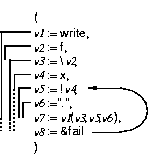
\includegraphics[width=1.7252in,height=1.6866in]{kw/figure4-1.png}  
%-%  \par}

\begin{center}
 \begin{tikzpicture}[>=latex, ultra thick,
      node distance= 1mm and 1mm,
      every label/.style={font=\small\it}
    ]
\node (t) {(};
\node (v1) [below=of t.south west, label=right:{v1 := {\tt write},}] {};
\node (v2) [below=of v1, label=right:{v2 := {\tt f},}] {};
\node (v3) [below=of v2, label=right:{v3 := {\tt \textbackslash}v2,}] {};
\node (v4) [below=of v3, label=right:{v4 := {\tt x},}] {};
\node (v5) [below=of v4, label=right:{v5 := {\tt !}v4,}] {};
\node (v6) [below=of v5, label=right:{v6 := {\tt \".\"},}] {};
\node (v7) [below=of v6, label=right:{v7 := v1(v3,v5,v6),}] {};
\node (v8) [below=of v7, label=right:{v8 := {\tt \&{}fail}}] {};
\node (b)  [below=of v8.south east] {)};

\draw (v1.west) -| ($(v7.west) - (1.2cm,0)$);
\draw (v2.west) -| ($(v3.west) - (1.0cm,0)$);
\draw (v3.west) -| ($(v7.west) - (0.8cm,0)$);
\draw (v4.west) -| ($(v5.west) - (0.6cm,0)$);
\draw (v5.west) -| ($(v7.west) - (0.4cm,0)$);
\draw (v6.west) -| ($(v7.west) - (0.2cm,0)$);
\begin{scope}[dotted]
\draw ($(v7.west) - (1.2cm,0)$) -- ($(v8.west) - (1.2cm,0)$);
\draw ($(v7.west) - (0.8cm,0)$) -- ($(v8.west) - (0.8cm,0)$);
\draw ($(v5.west) - (0.6cm,0)$) -- ($(v8.west) - (0.6cm,0)$);
\end{scope}

\draw[thick,->] ($(v8.east) + (2.2cm,0)$)
   to[out=0, in=0, distance= 3cm] ($(v5.east) + (2.2cm,0)$);
\end{tikzpicture}
\end{center}

Whether or not the program variables and constants are actually placed
in temporary variables depends on the machine model, implementation
conventions, and what optimizations are performed. Clearly a temporary
variable is not needed for \texttt{\&fail}. However, temporary variables are
needed if the subexpressions are more complex; intermediate values are
shown for all subexpressions for explanatory purposes.

When \texttt{\&fail} is executed, the \texttt{!} operation is
resumed. This creates an implicit loop from the \texttt{!} to
\texttt{\&fail}, as shown by the arrow in the above diagram. The
question is: What intermediate values must be retained up to
\texttt{\&fail}? A more instructive way to phrase the question is:
After \texttt{\&fail} is executed, what intermediate values could be
reused without being recomputed? From the sequence of primitive
operations, it is clear that the reused values include \textit{v1} and
\textit{v3}, and, if the element generation operator, \texttt{!},
references its argument after resumption, then the reused values
include \textit{v4}.\textit{ v2} is not used within the loop,
\textit{v5} and \textit{v6} are recomputed within the loop, and
\textit{v7} and \textit{v8} are not used. The lines in the diagram to
the left of the code indicate the lifetime of the intermediate
values. The dotted portion of each line represents the region of the
lifetime beyond what would exist in the absence of backtracking.

Liveness information could be computed by making the implicit loops
explicit then performing a standard liveness analysis in the form of a
global data flow analysis. That is unnecessarily expensive. There is
enough structure in this particular liveness problem that it can be
solved during the simple analysis required to locate the implicit
loops caused by goal-directed evaluation.

Several concepts are needed to describe analyses involving execution
order within Icon expressions. \textit{Forward execution order} is the
order in which operations would be executed at run time in the absence
of goal-directed evaluation and explicit loops. Goal-directed
evaluation involves both failure and the resumption of suspended
generators. The control clause of an \texttt{if-then-else} expression may fail,
but instead of resuming a suspending generator, it causes the \texttt{else}
clause to be executed. This failure results in forward execution
order. Forward execution order imposes a partial ordering on
operations. It produces no ordering between the \texttt{then} and the \texttt{else}
clauses of an \texttt{if} expression. \textit{Backtracking order} is the
reverse of forward execution order. This is due to the LIFO resumption
of suspended generators. The backward flow of control caused by
looping control structures does not contribute to this liveness
analysis (intermediate results used within a looping control structure
are also computed within the loop), but is dealt with in later
chapters. The \texttt{every} control structure is generally viewed as a looping
control structure.  However, it simply introduces failure. Looping
only occurs when it is used with a generative control clause, in which
case the looping is treated the same as goal-directed evaluation.

A notation that emphasizes intermediate values, subexpressions, and
execution order is helpful for understanding how liveness is
computed. Both postfix notation and syntax trees are inadequate. A
postfix notation is good for showing execution order, but tends to
obscure subexpressions. The syntax tree of an expression shows
subexpressions, but execution order must be expressed in terms of a
tree walk. In both representations, intermediate values are implicit.
For this discussion, an intermediate representation is used. A
subexpression is represented as a list of explicit intermediate values
followed by the operation that uses them, all enclosed in ovals. Below
each intermediate value is the subexpression that computes it. This
representation is referred to as a \textit{postfix tree}. The postfix
tree for the example above is:

%-% {\centering\color{green}
%-%  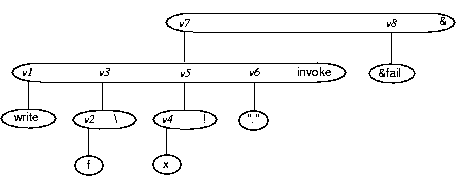
\includegraphics[width=5.1098in,height=1.9366in]{kw/figure4-2.png}  
%-% \par}

\begin{center}
\begin{tikzpicture} [thick,font=\it,
     rr/.style={rounded rectangle, fill=white, draw, minimum height=6mm, anchor=west}
   ]
% Use a matrix to establish positions, then paint stuff on top
\matrix [column sep=6mm, row sep=10mm]{
&&&&&&\node(v7){};&&&&&&&&\node(v8){};&&\node(amp){};\\
\node(v1){};&&&\node(v3){};&&&\node(v5){};&&&\node(v6){};&&\node(invoke){};&&&\node(fail){};&&\\
\node(write){};&&\node(v2){};&\node(v2c){};&\node(bslash){};&\node(v4){};&\node(v4c){};&
      \node(shriek){};&&\node(dot){};&&&&&&&&\\
&&\node(f){};&&&\node(x){};&&&&&&&&&&&\\
};
% Paint lines before filled rectangles before labels so the masking works.
\draw (v7) -- (v5) (v8) -- (fail);
\draw (v1) -- (write) (v3) -- (v2c) (v5) -- (v4c) (v6) -- (dot);
\draw (v2) -- (f) (v4) -- (x);
% Paint round rectangles
\node[rr, minimum width=9cm] at ($(v7.west) - (0.5cm,0)$) {};
\node[rr, minimum width=10.5cm] at ($(v1.west) - (0.5cm,0)$) {};
\foreach \n in {dot,f,x} {\node[rr, minimum width=1cm] at ($(\n.west) - (0.25cm,0)$) {};};
\foreach \n in {fail,write} {\node[rr, minimum width=1.5cm] at ($(\n.west) - (0.5cm,0)$) {};};
\foreach \n in {v2,v4} {\node[rr, minimum width=2.6cm] at ($(\n.west) - (0.2cm,0)$) {};};
% Paint labels
\foreach \n in {v7,v8,v1,v3,v5,v6,v2,v4} {\node at (\n) {\n};};
\foreach \n in {invoke,write,f,x} {\node at (\n) {\tt\small \n};};
\node at (amp) {\tt\small \&};
\node at (fail) {{\tt\small \&{}fail}};
\node[anchor=east] at (bslash) {\textbackslash};
\node[anchor=east] at (shriek) {\tt\small !};
\node at (dot) {\".\"};
\end{tikzpicture}
\end{center}

In this notation, the forward execution order of operations (which
includes constants and references to program variables) is
left-to-right and the backtracking order is right-to-left. In this
example, the backtracking order is \texttt{\&fail}, \texttt{invoke},
\texttt{"."}, \texttt{!}, \texttt{x}, \texttt{\textbackslash},
\texttt{f}, and \texttt{write}.

As explained above, the use of an intermediate value must appear in an
implicit loop for the value to have an extended lifetime. Two events
are needed to create such a loop. First, an operation must fail,
initiating backtracking. Second, an operation must be resumed, causing
execution to proceed forward again. This analysis computes the maximum
lifetime of intermediate values in the expression, so it only needs to
compute the rightmost operation (within a bounded expression) that can
fail. This represents the end of the farthest reaching loop. Once
execution proceeds beyond this point, no intermediate value can be
reused.

The intermediate values of a subexpression are used at the end of the
subexpression. For example, invoke uses the intermediate values
\textit{v1}, \textit{v3}, \textit{v5}, and \textit{v6}; the following
figure shows these intermediate results and the operation in
isolation.

%-% {\centering\color{green}
%-%  
\includegraphics[width=2.4937in,height=0.3402in]{kw/figure4-3.png}  
%-% \par}

\begin{center}
\begin{tikzpicture} [thick,
     rr/.style={rounded rectangle, fill=white, draw, minimum height=6mm, anchor=west}
   ]
% Use a matrix to establish positions, then paint stuff on top
\matrix [column sep=6mm, row sep=10mm]{
\node(v1){};&&&\node(v3){};&&&\node(v5){};&&&\node(v6){};&&\node(invoke){};\\
};
\node[rr, minimum width=10cm] at ($(v1.west) - (0.5cm,0)$) {};
\foreach \n in {v1,v3,v5,v6} {\node at (\n) {\it \n};};
\node[anchor=west] at (invoke) {\tt\small invoke};
\end{tikzpicture}
\end{center}

In order for these uses to be in a loop, backtracking must be
initiated from outside; that is, beyond the subexpression (in the
example, only \texttt{\&fail} and \texttt{\&} are beyond the subexpression).

In addition, for an intermediate value to have an extended lifetime,
the beginning of the loop must start after the intermediate value is
computed. Two conditions may create the beginning of a loop. First,
the operation itself may be resumed. In this case, execution continues
forward within the operation. It may reuse any of its operands and
none of them are recomputed. The operation does not have to actually
generate more results. For example, reversible swap (the operator
{\textless}--{\textgreater}) can be resumed to reuse both of its
operands, but it does not generate another result. Whether an
operation actually reuses its operands on resumption depends on its
implementation. In the Icon compiler, operations implemented with a C
function using the standard calling conventions always use copies of
operands on resumption, but implementations tailored to a particular
use often reference operand locations on resumption.  Liveness
analysis is presented here as if all operations reuse their operands
on resumption. In the actual implementation, liveness analysis
computes a separate lifetime for values used internally by operations
and the code generator decides whether this lifetime applies to
operands. This internal lifetime may also be used when allocating
tended descriptors for variables declared local to the in-line code
for an operation. The behavior of the temporary-variable model
presented in this dissertation can be compared with one developed by
Nilsen and Martinek [.martinek.]; it also relies on the liveness
analysis described in this chapter.

The second way to create the beginning of a loop is for a
subexpression to generate results. Execution continues forward again
and any intermediate values to the left of the generative
subexpression may be reused without being recomputed.  Remember,
backtracking is initiated from outside the expression. Suppose an
expression that can fail is associated with \textit{v6}, in the
previous figure. This creates a loop with the generator associated
with \textit{v5}. However, this particular loop does not include
invoke and does not contribute to the reuse of \textit{v1} or
\textit{v3}.

A resumable operation and generative subexpressions are all
\textit{resumption points} within an expression. A simple rule can be
used to determine which intermediate values of an expression have
extended lifetimes: If the expression can be resumed, the intermediate
values with extended lifetimes consist of those to the left of the
rightmost resumption point of the expression. This rule refers to the
{\textasciigrave}{\textasciigrave}top level'{}' intermediate values.
The rule must be applied recursively to subexpressions to determine
the lifetime of lower level intermediate values.

It sometimes may be necessary to make conservative estimates of what
can fail and of resumption points (for liveness analysis, it is
conservative to overestimate what can fail or be resumed). For
example, invocation may or may not be resumable, depending on what is
being invoked and, in general, it cannot be known until run time what
is being invoked (for the purposes of this example analysis, it is
assumed that the variable write is not changed anywhere in the
program).

In the example, the rightmost operation that can fail is
\texttt{\&fail}. Resumption points are \texttt{!} and the
subexpressions corresponding to the intermediate values \textit{v5}
and \textit{v7}.

Once the resumption points have been identified, the rule for
determining extended lifetimes can be applied. If there are no
resumption points in an expression, no intermediate values in that
expression can be reused. Applying this rule to the postfix tree above
yields \textit{v1}, \textit{v3}, and \textit{v4} as the intermediate
values that have extended lifetimes.

Similar techniques can be used for liveness analysis of Prolog
programs, where goal-directed evaluation also creates implicit
loops. One difference is that a Prolog clause is a linear sequence of
calls. It does not need to be ``linearized'' by constructing a
postfix tree. Another difference is that all intermediate values in
Prolog programs are stored in explicit variables. A Prolog variable
has a lifetime that extends to the right of its last use if an
implicit loops starts after the variable's first use and ends after
the variable's last use.


\section[16.3 An Attribute Grammar]{16.3 An Attribute Grammar}

To cast this approach as an attribute grammar, an expression should be
thought of in terms of an abstract syntax tree.  The transformation
from a postfix tree to a syntax tree is trivial. It is accomplished by
deleting the explicit intermediate values. A syntax tree for the
example is:

%-% 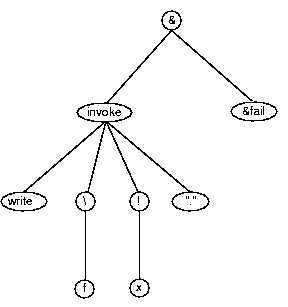
\includegraphics[width=3.1638in,height=3.198in]{kw/figure4-4.png}

\begin{center}
\begin{tikzpicture} [thick,font=\small\tt,
     rr/.style={rounded rectangle, fill=white, draw, minimum height=6mm}
   ]

\node (root) [rr] {\&}
  child
  { node[rr]{invoke}
    child { node [rr] {write} }
    child { node [rr] {\textbackslash}
            child { node[rr] {f}}
          }
    child { node [rr] {!} child { node[rr] {x} } }
    child {node [rr] {"."} }
  }
  child[missing]
  child { node[rr] {\&{}fail} };
\end{tikzpicture}
\end{center}

Several interpretations can be given to a node in a syntax tree. A
node can be viewed as representing either an operation, an entire
subexpression, or an intermediate value.

This analysis associates four attributes with each node (this ignores
attributes needed to handle \texttt{break} expressions).  The goal of
the analysis is to produce the \texttt{lifetime} attribute. The other
three attributes are used to propagate information needed to compute
the \texttt{lifetime}.

\liststyleLxix
\begin{itemize}

\item \texttt{resumer} is either the rightmost operation (represented
as a node) that can initiate backtracking into the subexpression or it
is null if the subexpression cannot be resumed.

\item \texttt{failer} is related to \texttt{resumer}. It is the
rightmost operation that can initiate backtracking that can continue
past the subexpression. It is the same as \texttt{resumer}, unless the
subexpression itself contains the rightmost operation that can fail.

item \texttt{gen} is a boolean attribute. It is true if the
subexpression can generate multiple results if resumed.

\item \texttt{lifetime} is the operation beyond which the intermediate
value is no longer needed. It is either the parent node, the
\texttt{resumer} of the parent node, or null. The \texttt{lifetime} is
the parent node if the value is never reused after execution leaves
the parent operation. The \texttt{lifetime} is the \texttt{resumer} of
the parent if the parent operation or a generative sibling to the
right can be resumed. A lifetime of null is used to indicate that the
intermediate value is never used. For example, the value of the
control clause of an \texttt{if} expression is never used.

\end{itemize}

Attribute computations are associated with productions in the
grammar. The attribute computations for \texttt{failer} and
\texttt{gen} are always for the non-terminal on the left-hand side of
the production. These values are then used at the parent production;
they are effectively passed up the syntax tree. The computations for
\texttt{resumer} and \texttt{lifetime} are always for the attributes
of non-terminals on the right-hand side of the
production. \texttt{resumer} is then used at the productions defining
these non-terminals; it is effectively passed down the syntax
tree. \texttt{lifetime} is usually saved just for the code generator,
but it is sometimes used by child nodes.


\section[16.4 Primary Expressions]{16.4 Primary Expressions}

Variables, literals, and keywords are primary expressions. They have
no subexpressions, so their productions contain no computations for
\texttt{resumer} or \texttt{lifetime}. The attribute computations for
a literal follow. A literal itself cannot fail, so backtracking only
passes beyond it if the backtracking was initiated before (to the
right of) it. A literal cannot generate multiple results.

\goodbreak
\begin{iconcode}
\>expr ::= literal \>\>\>\>\ \{\\
\>\>\>\>\>\>expr.failer := expr.resumer\\
\>\>\>\>\>\>expr.gen := false\\
\>\>\>\>\>\ \}\\
\end{iconcode}



Another example of a primary expression is the keyword
\texttt{\&fail}. Execution cannot continue past \texttt{\&fail}, so it
must be the rightmost operation within its bounded expression that can
fail. A pre-existing attribute, \texttt{node}, is assumed to exist for
every symbol in the grammar. It is the node in the syntax tree that
corresponds to the symbol.

\goodbreak
\begin{iconcode}
\>expr ::= \&fail\>\>\>\> \{\\
\>\>\>\>\>\>expr.failer := expr.node\\
\>\>\>\>\>\>expr.gen := false\\
\>\>\>\>\>\}\\
\end{iconcode}


\section[16.5 Operations with Subexpressions]{16.5 Operations with Subexpressions}

Addition provides an example of the attribute computations involving
subexpressions. The following diagram shows how \texttt{resumer},
\texttt{failer}, and \texttt{gen} information would be passed through
the postfix tree.

%-% \noindent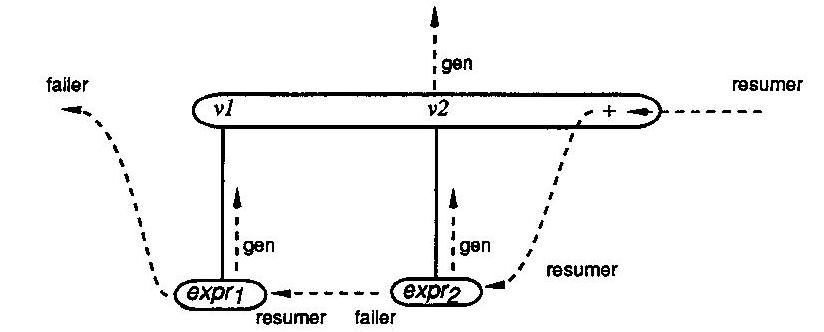
\includegraphics[width=5.9in,height=2.3in]{kw/figure4-5.png}

\begin{center}
\begin{tikzpicture} [thick,>=latex, font=\small\tt,
     rr/.style={rounded rectangle, fill=white, draw, minimum height=6mm, anchor=west}
   ]
% Use a matrix to establish positions, then paint stuff on top
\matrix [column sep=20mm, row sep=20mm]{
&[5mm]&[20mm]\node(outT){};&[5mm]&\\[-3mm]
\node(outL){};&\node(v1){};&\node(v2){};&\node(pl){};&\node(inR){};\\[5mm]
&\node(ex1){};&\node(ex2){};&&\\
};
% Draw these lines before, so the rectangle shape masks them
\draw [dashed,->] (v2) to node[right] {gen} (outT);
\draw (ex1) -- (v1) (ex2) -- (v2);
\foreach \p in {ex1,ex2} {
  \draw [dashed,->] ($(\p) + (0.3cm,0)$) to node[right] {gen} ($(\p) + (0.3cm,1.7cm)$);
};
\node[rr, minimum width=9cm] at ($(v1.west) - (0.7cm,0)$) {};
\foreach \n in {v1,v2} {\node at (\n) {\it \n};};
\node (plus) at (pl) {+};
\node (expr1) [rr,anchor=center] at (ex1) {expr$_1$};
\node (expr2) [rr,anchor=center] at (ex2) {expr$_2$};
\draw [dashed,->] (plus.west) to[out=180,in=0] node[near end, right] {~resumer} (expr2.east);
\draw [dashed,->] (inR) -- (plus.east);
\node [above] at (inR) {resumer};
\draw [dashed,->] (expr2.west) to node[below]{resumer\hspace{0.7cm}failer} (expr1.east);
\draw [dashed,->] (expr1.west) to[out=180,in=0] (outL);
\node [above] at (outL) {failer};
\end{tikzpicture}
\end{center}

This information would then be used to compute \texttt{lifetime}
information for \textit{v1} and \textit{v2}. The next figure shows how
the attribute information is actually passed through the syntax tree.

%-% 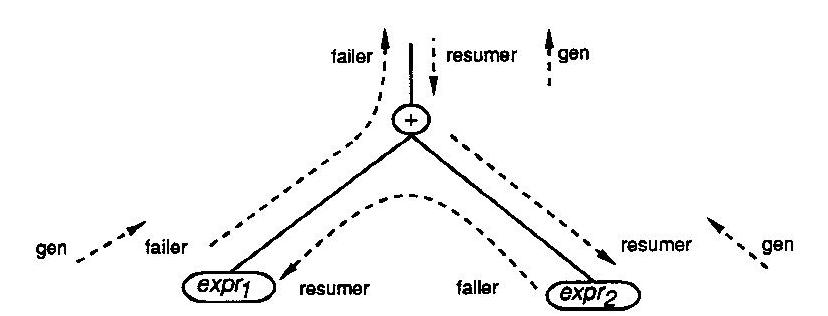
\includegraphics[width=6.0in,height=2.2in]{kw/figure4-6.png}  

\begin{center}
\begin{tikzpicture} [draw,thick,>=latex, font=\small\tt,
     rr/.style={rounded rectangle, fill=white, draw, minimum height=6mm}
   ]
% Draw the nodes
\node (pl) [rr] at (5,4) {+};
\node (e1) [rr] at (2,1) {expr$_1$};
\node (e2) [rr] at (8,1) {expr$_2$};
% connect the nodes
\draw (5,4.75) -- (pl) -- (e1) (pl) -- (e2);
% draw failer and resumer lines
\draw[dashed,->] (1.5,1.5) -- (4,4) to[in=270] (4.5,5) node[at start, left] {failer};
\draw[dashed,->] (5.5,5) -- ($(pl) + (0.5,0)$) node[at start, right] {resumer};
\node[xshift=0.5cm,anchor=east] at (4,5) {failer};
\draw[dashed,->] (6,3.5) -- ($(e2) + (0,0.5)$) node[at end,right] {resumer};
% Now the complicated bit: draw a nice bendy line between e2 and e1
\draw[dashed,->] ($(e2.west)+(0,0.25)$)
   .. controls (6,3) and (4,3)
   .. ($(e1.east)+(0,0.25)$)
   node[at start,left] {failer~} node[at end, right] {~resumer};
% Draw the "gen" lines
\draw[dashed,->] (8,4) -- (8,5) node[at end,right] {gen};
\draw[dashed,->] (10.5,1.5) -- (9.5,2.5) node[at start,right] {gen};
\draw[dashed,->] (-0.5,1.5) -- (0.5,2.5) node[at start,left] {gen};
\end{tikzpicture}
\end{center}

\noindent
The \texttt{lifetime} attributes are computed for the roots of the
subtrees for \texttt{expr}\TextSubscript{1} and
\texttt{expr}\TextSubscript{2}.


The details of the attribute computations depend, in part, on the
characteristics of the individual operation. Addition does not fail,
so the rightmost resumer, if there is one, of
\texttt{expr}\TextSubscript{2} is the rightmost resumer of the entire
expression. The rightmost resumer of \texttt{expr}\TextSubscript{1} is
the rightmost operation that can initiate backtracking that continues
past \texttt{expr}\TextSubscript{2}. Addition does not suspend, so the
lifetime of the value produced by \texttt{expr}\TextSubscript{2} only
extends through the operation (that is, it always is recomputed in the
presence of goal-directed evaluation). If
\texttt{expr}\TextSubscript{2} is a generator, then the result of
\texttt{expr}\TextSubscript{1} must be retained for as long as
\texttt{expr}\TextSubscript{2} might be resumed. Otherwise, it need
only be retained until the addition is
performed. \texttt{expr}\TextSubscript{1} is the first thing executed
in the expression, so its \texttt{failer} is the \texttt{failer} for
the entire expression. The expression is a generator if either
\texttt{expr}\TextSubscript{1} or \texttt{expr}\TextSubscript{2} is a
generator (note that the operation {\textbar} is logical \textit{or},
not Icon's alternation control structure):

\goodbreak
\begin{iconcode}
\>expr ::= expr\TextSubscript{1} + expr\TextSubscript{2} \{\\
\>\>\>\>\>expr\TextSubscript{2}.resumer := expr.resumer\\
\>\>\>\>\>expr\TextSubscript{2}.lifetime := expr.node\\
\>\>\>\>\>expr\TextSubscript{1}.resumer := expr\TextSubscript{2}.failer\\
\>\>\>\>\>if expr\TextSubscript{2}.gen \& (expr.resumer ${\neq}$ null) then\\
\>\>\>\>\>\>expr\TextSubscript{1}.lifetime := expr.resumer\\
\>\>\>\>\>else\\
\>\>\>\>\>\>expr\TextSubscript{1}.lifetime := expr.node\\
\>\>\>\>\>expr.failer := expr\TextSubscript{1}.failer\\
\>\>\>\>\>expr.gen := (expr\TextSubscript{1}.gen | expr\TextSubscript{2}.gen)\\
\>\>\>\>\>\}\\
\end{iconcode}


\texttt{/expr} provides an example of an operation that can fail. If
there is no rightmost resumer of the entire expression, it is the
rightmost resumer of the operand. The lifetime of the operand is
simply the operation, by the same argument used for
\texttt{expr}\TextSubscript{2} of addition. The computation of
\texttt{failer} is also analogous to that of addition. The expression
is a generator if the operand is a generator:

\goodbreak
\begin{iconcode}
\>expr ::= /expr\TextSubscript{1} \{\\
\>\>\>\>if expr.resumer = null then\\
\>\>\>\>\>expr\TextSubscript{1}.resumer := expr.node\\
\>\>\>\>else\\
\>\>\>\>\>expr\TextSubscript{1}.resumer := expr.resumer\\
\>\>\>\>expr\TextSubscript{1}.lifetime := expr.node\\
\>\>\>\>expr.failer := expr\TextSubscript{1}.failer\\
\>\>\>\>expr.gen := expr\TextSubscript{1}.gen\\
\>\>\>\>\}\\
\end{iconcode}


\texttt{!expr} differs from \texttt{/expr} in that it can generate
multiple results. If it can be resumed, the result of the operand must
be retained through the rightmost \texttt{resumer}:

\goodbreak
\begin{iconcode}
\>expr ::= !expr\TextSubscript{1} \{\\
\>\>\>\>if expr.resumer = null then \{\\
\>\>\>\>\>expr\TextSubscript{1}.resumer := expr.node\\
\>\>\>\>\>expr\TextSubscript{1}.lifetime := expr.node\\
\>\>\>\>\>\}\\
\>\>\>\>else \{\\
\>\>\>\>\>expr\TextSubscript{1}.resumer := expr.resumer\\
\>\>\>\>\>expr\TextSubscript{1}.lifetime := expr.resumer\\
\>\>\>\>\>\}\\
\>\>\>\>expr.failer := expr\TextSubscript{1}.failer\\
\>\>\>\>expr.gen := true\\
\>\>\>\>\}\\
\end{iconcode}


\section[16.6 Control Structures]{16.6 Control Structures}

Other operations follow the general pattern of the ones presented
above. Control structures, on the other hand, require unique attribute
computations. In particular, several control structures bound
subexpressions, limiting backtracking.  For example, \texttt{not}
bounds its argument and discards the value. If it has no
\texttt{resumer}, then it is the rightmost operation that can
fail. The expression is not a generator:

\goodbreak
\begin{iconcode}
\>expr ::= not expr\TextSubscript{1} \{\\
\>\>\>\>expr\TextSubscript{1}.resumer := null\\
\>\>\>\>expr\TextSubscript{1}.lifetime := null\\
\>\>\>\>if expr.resumer = null then\\
\>\>\>\>\>expr.failer := expr.node\\
\>\>\>\>else\\
\>\>\>\>\>expr.failer := expr.resumer\\
\>\>\>\>expr.gen := false\\
\>\>\>\>\}\\
\end{iconcode}


\texttt{expr}\TextSubscript{1} \texttt{; expr}\TextSubscript{2} bounds
\texttt{expr}\TextSubscript{1} and discards the result. Because the
result of \texttt{expr}\TextSubscript{2} is the result of the entire
expression, the code generator makes their result locations
synonymous. This is reflected in the lifetime computations. Indeed,
all the attributes of \texttt{expr}\TextSubscript{2} and those of the
expression as a whole are the same:

\goodbreak
\begin{iconcode}
\>expr ::= expr\TextSubscript{1} ; expr\TextSubscript{2} \{\\
\>\>\>\>\>expr\TextSubscript{1}.resumer := null\\
\>\>\>\>\>expr\TextSubscript{1}.lifetime := null\\
\>\>\>\>\>expr\TextSubscript{2}.resumer := expr.resumer\\
\>\>\>\>\>expr\TextSubscript{2}.lifetime := expr.lifetime\\
\>\>\>\>\>expr.failer := expr\TextSubscript{2}.failer\\
\>\>\>\>\>expr.gen := expr\TextSubscript{2}.gen\\
\>\>\>\>\>\}\\
\end{iconcode}


A reasonable implementation of alternation places the result of each
subexpression into the same location: the location associated with the
expression as a whole. This is reflected in the lifetime
computations. The resumer of the entire expression is also the resumer
of each subexpression. Backtracking out of the entire expression
occurs when backtracking out of \texttt{expr}\TextSubscript{2}
occurs. This expression is a generator:

\goodbreak
\begin{iconcode}
\>expr ::= expr\TextSubscript{1} | expr\TextSubscript{2} \{\\
\>\>\>\>\>expr\TextSubscript{2}.resumer:= expr.resumer\\
\>\>\>\>\>expr\TextSubscript{2}.lifetime := expr.lifetime\\
\>\>\>\>\>expr\TextSubscript{1}.resumer := expr.resumer\\
\>\>\>\>\>expr\TextSubscript{1}.lifetime := expr.lifetime\\
\>\>\>\>\>expr.failer := expr\TextSubscript{2}.failer\\
\>\>\>\>\>expr.gen := true\\
\>\>\>\>\>\}\\
\end{iconcode}


The first operand of an \texttt{if} expression is bounded and its
result is discarded. The other two operands are treated similar to
those of alternation. Because there are two independent execution
paths, the rightmost resumer may not be well-defined. However, it is
always conservative to treat the resumer as if it is farther right
than it really is; this just means that an intermediate value is kept
around longer than needed. If there is no resumer beyond the
\texttt{if} expression, but at least one of the branches can fail, the
failure is treated as if it came from the end of the \texttt{if}
expression (represented by the node for the expression). Because
backtracking out of an \texttt{if} expression is rare, this inaccuracy
is of little practical consequence. The \texttt{if} expression is a
generator if either branch is a generator:

\goodbreak
\begin{iconcode}
\>expr ::= if expr\TextSubscript{1} then expr\TextSubscript{2}~%
                                    else expr\TextSubscript{3} \{\\
\>\>\>\>\>expr\TextSubscript{3}.resumer := expr.resumer\\
\>\>\>\>\>expr\TextSubscript{3}.lifetime := expr.lifetime\\
\>\>\>\>\>expr\TextSubscript{2}.resumer := expr.resumer\\
\>\>\>\>\>expr\TextSubscript{2}.lifetime := expr.lifetime\\
\>\>\>\>\>expr\TextSubscript{1}.resumer := null\\
\>\>\>\>\>expr\TextSubscript{1}.lifetime := null\\
\>\>\>\>\>if expr.resumer = null \& (expr\TextSubscript{1}.failer $\neq$ null |~%
                                  expr\TextSubscript{2}.failer $\neq$ null) then\\
\>\>\>\>\>\>expr.failer := expr.node\\
\>\>\>\>\>else\\
\>\>\>\>\>\>expr.failer = expr.resumer\\
\>\>\>\>\>expr.gen := (expr\TextSubscript{2}.gen | expr\TextSubscript{3}.gen)\\
\>\>\>\>\>\}\\
\end{iconcode}


The \texttt{do} clause of \texttt{every} is bounded and its result
discarded. The control clause is always resumed at the end of the loop
and can never be resumed by anything else. The value of the control
clause is discarded. Ignoring \texttt{break} expressions, the loop
always fails:

\goodbreak
\begin{iconcode}
\>expr ::= every expr\TextSubscript{1} do expr\TextSubscript{2} \{\\
\>\>\>\>\>expr\TextSubscript{2}.resumer := null\\
\>\>\>\>\>expr\TextSubscript{2}.lifetime := null\\
\>\>\>\>\>expr\TextSubscript{1}.resumer := expr.node\\
\>\>\>\>\>expr\TextSubscript{1}.lifetime := null\\
\>\>\>\>\>expr.failer := expr.node\\
\>\>\>\>\>expr.gen := false\\
\>\>\>\>\>\}\\
\end{iconcode}


Handling \texttt{break} expressions requires some stack-like
attributes. These are similar to the ones used in the control flow
analyses described in O'Bagy's dissertation [.tr88-31.] and the ones
used to construct flow graphs in the original technical report on type
inferencing.

The attributes presented here can be computed with one walk of the
syntax tree. At a node, subtrees are processed in reverse execution
order: first the \texttt{resumer} and \texttt{lifetime} attributes of
a subtree are computed, then the subtree is walked. Next the
\texttt{failer} and \texttt{gen} attributes for the node itself are
computed, and the walk moves back up to the parent node.
